\whiteBGstarBegin
\setcounter{section}{0}
\section{Trắc nghiệm}
\begin{enumerate}[label=\bfseries Câu \arabic*:]
	
	
	\item \mkstar{1}
	
	\cauhoi
	{Công của lực điện trường làm dịch chuyển điện tích $Q$ từ điểm A đến điểm B trong điện trường sẽ phụ thuộc vào
		\begin{mcq}
			\item tọa độ của A và B.
			\item chiều dài quãng đường điện tích di chuyển từ A tới B.
			\item quỹ đạo đi từ A đến B.
			\item khoảng cách AB.
		\end{mcq}
		
	}
	\loigiai
	{	\textbf{Đáp án: A.}
		
		Công của lực điện chỉ phụ thuộc vào tọa độ của điểm đầu và điểm cuối.
	}
	\item \mkstar{1}
	
	\cauhoi
	{Phát biểu nào sau đây về công của lực điện trường là \textbf{không} đúng?
		\begin{mcq}
			\item Khi điện tích chuyển động trên đường thẳng vuông góc với đường sức điện thì công của lực điện trường bằng 0.
			\item Công của lực điện trường phụ thuộc vào hình dạng quỹ đạo chuyển động.
			\item Công của lực điện trường phụ thuộc vào điểm đầu và điểm cuối của quỹ đạo chuyển động.
			\item Công của lực điện trường trên đường cong kín bằng 0.
		\end{mcq}
		
	}
	\loigiai
	{	\textbf{Đáp án: B.}
		
		Công của lực điện trường không phụ thuộc vào hình dạng quỹ đạo chuyển động, mà chỉ phụ thuộc vào điểm đầu và điểm cuối.
	}
	\item \mkstar{2}
	
	\cauhoi
	{Công của lực điện trường dịch chuyển một điện tích $\SI{1}{\micro C}$ dọc theo chiều một đường sức điện trong điện trường đều có độ lớn cường độ điện trường $\SI{1000}{V/m}$ trên quãng đường dài $\SI{1}{m}$ là
		\begin{mcq}(4)
			\item $\SI{1}{mJ}$.
			\item 1 J.
			\item 1000 J.
			\item $\SI{1}{\micro J}$.
		\end{mcq}
		
	}
	\loigiai
	{	\textbf{Đáp án: A.}
		
		Công của lực điện:
		$$A=qEd=\SI{1}{mJ}.$$
	}
	\item \mkstar{2}
	
	\cauhoi
	{Công của lực điện trường khác 0 khi điện tích dịch chuyển như thế nào?
		\begin{mcq}
			\item Dịch chuyển giữa 2 điểm khác nhau cắt các đường sức.
			\item Dịch chuyển vuông góc với các đường sức trong điện trường đều.
			\item Dịch chuyển hết quỹ đạo là đường cong kín trong điện trường.
			\item Dịch chuyển hết một quỹ đạo tròn trong điện trường.
		\end{mcq}
		
	}
	\loigiai
	{	\textbf{Đáp án: A.}
		
		Công của lực điện trường khác 0 khi điện tích dịch chuyển giữa 2 điểm khác nhau cắt các đường sức.
		
		Các trường hợp còn lại đều có $A=0$.
	}
	\item \mkstar{2}
	
	\cauhoi
	{Một điện tích điểm $q$ di chuyển từ điểm M đến điểm N trong điện trường đều như hình vẽ.
		\begin{center}
			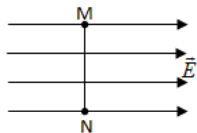
\includegraphics{../figs/VN11-2021-PH-TP005-1}
		\end{center}
	Khẳng định nào sau đây đúng?
		\begin{mcq}
			\item Lực điện trường thực hiện công dương.
			\item Lực điện trường thực hiện công âm.
			\item Lực điện trường không thực hiện công.
			\item Không xác định được công của lực điện trường.
		\end{mcq}
		
	}
	\loigiai
	{	\textbf{Đáp án: C.}
		
		Điện tích dịch chuyển vuông góc với các đường sức nên công của lực điện trường bằng 0.
	}
	\item \mkstar{2}
	
	\cauhoi
	{Khi điện tích dịch chuyển dọc theo một đường sức trong một điện trường đều, nếu quãng đường dịch chuyển tăng 2 lần thì công của lực điện trường
		\begin{mcq}(4)
			\item tăng 4 lần.
			\item tăng 2 lần.
			\item không đổi.
			\item giảm 2 lần.
		\end{mcq}
		
	}
	\loigiai
	{	\textbf{Đáp án: C.}
		
		Công của lực điện trường không phụ thuộc vào quãng đường dịch chuyển của điện tích giữa hai điểm trong điện trường.
	}
	\item \mkstar{2}
	
	\cauhoi
	{Công của lực điện khi di chuyển một điện tích điểm $q=\SI{2e-6}{C}$ qua hiệu điện thế $U=\SI{2}{V}$ có độ lớn là
		\begin{mcq}(4)
			\item $\SI{0.5e-6}{J}$.
			\item $\SI{e-6}{J}$.
			\item $\SI{2e-6}{J}$.
			\item $\SI{4e-6}{J}$.
		\end{mcq}
		
	}
	\loigiai
	{	\textbf{Đáp án: D.}
		
		Áp dụng công thức:
		$$A=qU=\SI{4e-6}{J}.$$
	}
	\item \mkstar{2}
	
	\cauhoi
	{Xác định công của lực điện trường khi di chuyển một electron từ điểm A đến điểm B. Biết hiệu điện thế giữa hai điểm A và B là $U=\SI{5}{V}$.
		\begin{mcq}(4)
			\item $A=\SI{-5}{eV}$.
			\item $A=\SI{5}{eV}$.
			\item $A=\SI{8e-18}{J}$.
			\item $A=\SI{-8e-18}{J}$.
		\end{mcq}
		
	}
	\loigiai
	{	\textbf{Đáp án: A.}
		
		Áp dụng công thức:
		$$A=qU=eU=e\cdot \SI{5}{V} = \SI{5}{eV}.$$
		
		Vì $U_\text{AB} > 0$ nên điện thế tại A cao hơn điện thế tại B, suy ra công của lực điện trường tác dụng lên electron khi nó dịch chuyển từ A đến B là công cản, vậy $A=\SI{-5}{eV}$.
	}
	\item \mkstar{2}
	
	\cauhoi
	{Một điện tích điểm $q$ chuyển động trong điện trường đều $E$ có quỹ đạo là một đường cong khép kín. Gọi chiều dài quỹ đạo là $s$ thì công của lực điện trường là
		\begin{mcq}(4)
			\item $A=2qEs$.
			\item $A=0$.
			\item $A=qEs$.
			\item $A=qE/s$.
		\end{mcq}
		
	}
	\loigiai
	{	\textbf{Đáp án: B.}
		
		Công của lực điện trường làm dịch chuyển một điện tích theo một đường cong khép kín bằng 0.
	}
	\item \mkstar{2}
	
	\cauhoi
	{Công của lực điện trường làm dịch chuyển một điện tích $\SI{-2}{\micro C}$ ngược chiều một đường sức trong điện trường đều có độ lớn $\SI{1000}{V/m}$ trên quãng đường dài $\SI{1}{m}$. Xác định công của lực điện trường trong trường hợp này.
		\begin{mcq}(4)
			\item $A=\SI{2000}{J}$.
			\item $A=\SI{-2000}{J}$.
			\item $A=\SI{2}{mJ}$.
			\item $A=\SI{-2}{mJ}$.
		\end{mcq}
		
	}
	\loigiai
	{	\textbf{Đáp án: C.}
		
		Vì điện tích $q<0$ nên khi dịch chuyển ngược chiều điện trường, công của lực điện tác dụng lên điện tích là công phát động ($A>0$).
		
		Áp dụng công thức:
		$$A=qEd  =\SI{2}{mJ}.$$
	}
	\item \mkstar{2}
	
	\cauhoi
	{Một electron di chuyển được một đoạn đường $\SI{1}{cm}$ dọc theo đường sức điện trong một điện trường đều có cường độ $\SI{1000}{V/m}$. Xác định công của lực điện trong dịch chuyển trên.
		\begin{mcq}(4)
			\item $\SI{-1.6e-18}{J}$.
			\item $\SI{1.6e-16}{J}$.
			\item $\SI{1.6e-18}{J}$.
			\item $\SI{-1.6e-16}{J}$.
		\end{mcq}
		
	}
	\loigiai
	{	\textbf{Đáp án: C.}
		
		Vì lực điện tác dụng lên electron cùng chiều với chiều dịch chuyển của electron nên sinh công dương.
		
		Áp dụng công thức:
		$$A=qEd=eEd = \SI{1.6e-18}{J}.$$
	}
	\item \mkstar{2}
	
	\cauhoi
	{Trong một điện trường đều cường độ $\SI{60000}{V/m}$ có điện tích $q_0=\SI{4e-9}{C}$ dịch chuyển trên đoạn thẳng dài $\SI{5}{cm}$. Biết góc giữa phương dịch chuyển và đường sức điện là $\alpha = 60^\circ$. Xác định công của lực điện trong trường hợp trên.
		\begin{mcq}(4)
			\item $\SI{e-6}{J}$.
			\item $\SI{6e6}{J}$.
			\item $\SI{6e-6}{J}$.
			\item $\SI{-6e-6}{J}$.
		\end{mcq}
		
	}
	\loigiai
	{	\textbf{Đáp án: C.}
		
		Áp dụng công thức:
		$$A=qEd=qEs \cos \alpha = \SI{6e-6}{J}.$$
	}
	\item \mkstar{2}
	
	\cauhoi
	{Công của lực điện trường làm dịch chuyển một điện tích $q>0$ một đoạn $d$ theo hướng của một đường sức điện trong điện trường đều có cường độ $E$ có biểu thức
		\begin{mcq}(4)
			\item $A=\dfrac{qE}{d}$.
			\item $A=qEd$.
			\item $A=-\dfrac{qE}{d}$.
			\item $A=-qEd$.
		\end{mcq}
		
	}
	\loigiai
	{	\textbf{Đáp án: B.}
		
		Vì điện tích dịch chuyển cùng chiều với lực điện nên công dương: $A=qEd$.
	}
	\item \mkstar{2}
	
	\cauhoi
	{Cho điện tích $q$ dịch chuyển giữa hai điểm cố định trong một điện trường đều có cường độ $\SI{150}{V/m}$ thì công của lực điện trường là $\SI{60}{mJ}$. Nếu cường độ điện trường là $\SI{200}{V/m}$ thì công của lực điện trường tương ứng là
		\begin{mcq}(4)
			\item $\SI{40}{J}$.
			\item $\SI{40}{mJ}$.
			\item $\SI{80}{J}$.
			\item $\SI{80}{mJ}$.
		\end{mcq}
		
	}
	\loigiai
	{	\textbf{Đáp án: D.}
		
		Lập tỉ lệ:
		$$\dfrac{A_1}{A_2} = \dfrac{E_1}{E_2} = \dfrac{3}{4} \Rightarrow A_2 = \SI{80}{mJ}.$$
	}
	\item \mkstar{2}
	
	\cauhoi
	{Khi điện tích dịch chuyển trong điện trường đều dọc theo chiều đường sức thì công của lực điện tác dụng lên nó là $\SI{10}{J}$. Cũng với điện tích ấy và khoảng cách dịch chuyển ấy, nếu chiều dịch chuyển hợp với chiều đường sức một góc $60^\circ$ thì công của lực điện là
		\begin{mcq}(4)
			\item $\SI{7.5}{J}$.
			\item $\xsi{\dfrac{5\sqrt{3}}{2}}{J}$.
			\item $\SI{5}{J}$.
			\item $\xsi{5\sqrt{2}}{J}$.
		\end{mcq}
		
	}
	\loigiai
	{	\textbf{Đáp án: C.}
		
		Lập tỉ lệ:
		$$\dfrac{A_1}{A_2} = \dfrac{\cos 0}{\cos 60^\circ} = 2 \Rightarrow A_2 = \SI{5}{J}.$$
	}
	\item \mkstar{3}
	
	\cauhoi
	{Dưới tác dụng của lực điện trường, một điện tích $q$ dương di chuyển được một đoạn đường $s$ trong điện trường đều theo phương hợp với $\vec E$ một góc $\alpha$. Trong trường hợp nào sau đây, công của lực điện trường là lớn nhất?
		\begin{mcq}(4)
			\item $\alpha = 0^\circ$.
			\item $\alpha=45^\circ$.
			\item $\alpha = 60^\circ$.
			\item $\alpha=90^\circ$.
		\end{mcq}
		
	}
	\loigiai
	{	\textbf{Đáp án: A.}
		
		Khi $\alpha = 0$ thì điện tích dịch chuyển theo phương đường sức, khi đó công của lực điện trường là lớn nhất.
	}
	\item \mkstar{3}
	
	\cauhoi
	{Cho điện tích thử $q$ di chuyển trong một điện trường đều dọc theo hai đoạn thẳng MN và NP. Biết rằng lực điện sinh công dương và MN dài hơn NP. Hỏi biểu thức nào sau đây là đúng?
		\begin{mcq}(2)
			\item $A_\text{MN} > A_\text{NP}$.
			\item $A_\text{MN} < A_\text{NP}$.
			\item $A_\text{MN} = A_\text{NP}$.
			\item Cả 3 biểu thức đều đúng.
		\end{mcq}
		
	}
	\loigiai
	{	\textbf{Đáp án: D.}
		
		Tùy thuộc vào góc $\alpha$ mà độ lớn công của lực điện khác nhau. Do đó cả 3 trường hợp đều có thể xảy ra.
	}
	\item \mkstar{3}
	
	\cauhoi
	{Công của lực điện trường dịch chuyển một điện tích điểm $q=\SI{5}{\micro C}$ đi từ điểm M đến điểm N ($\text{MN} = \SI{2}{cm}$) trong một điện trường đều có cường độ $E=\SI{e5}{V/m}$ là bao nhiêu? Biết $\overrightarrow{\text{MN}}$ vuông góc $\vec E$.
		\begin{mcq}(4)
			\item 1 J.
			\item 1000 J.
			\item 100 mJ.
			\item 0 J.
		\end{mcq}
		
	}
	\loigiai
	{	\textbf{Đáp án: D.}
		
		Do $\overrightarrow{\text{MN}}\ \bot \vec{E}$ nên $A=0$.
	}
	\item \mkstar{3}

	\cauhoi
	{Một ion hidro $\ce{H}^+$ được đặt vào trong một điện trường đều với cường độ điện trường $E=\SI{e4}{V/m}$. Khi ion hidro này dịch chuyển được $\SI{0.1}{mm}$ thì đã nhận được công của lực điện với giá trị là
		\begin{mcq}(4)
			\item $\SI{0}{J}$.
			\item $\SI{-1.6e-19}{J}$.
			\item $\SI{e-19}{J}$.
			\item $\SI{1.6e-19}{J}$.
		\end{mcq}
		
	}
	\loigiai
	{	\textbf{Đáp án: D.}
		
		Ion $\ce{H}^+$ có điện tích $q=+\SI{1.6e-19}{C}$.
		
		Đổi $d=\SI{0.1}{mm}=\SI{1e-4}{m}$
		
		Áp dụng công thức:
		$$A=qEd = \SI{1.6e-19}{J}.$$
	}
	\item \mkstar{4}
	
	\cauhoi
	{Một điện tích $q=\SI{4e-8}{C}$ di chuyển trong một điện trường đều có cường độ $E=\SI{100}{V/m}$ theo một đường gấp khúc ABC. Đoạn AB dài 20 cm và vectơ độ dời $\overrightarrow{\text{AB}}$ làm với các đường sức điện một góc $30^\circ$. Đoạn BC dài 40 cm và vectơ độ dời $\overrightarrow{\text{BC}}$ làm với các đường sức điện một góc $120^\circ$. Tính công của lực điện khi điện tích di chuyển từ A đến C.
		\begin{mcq}(4)
			\item $\SI{1.5e-6}{J}$.
			\item $\SI{-1.5e-6}{J}$.
			\item $\SI{0.1e-6}{J}$.
			\item $\SI{-0.1e-6}{J}$.
		\end{mcq}
		
	}
	\loigiai
	{	\textbf{Đáp án: D.}
		
		\begin{center}
			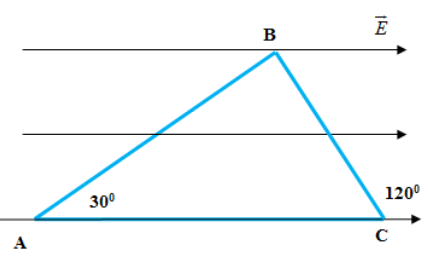
\includegraphics{../figs/VN11-2021-PH-TP005-2}
		\end{center}
	
	Công của lực điện trên đoạn AB:
	$$A_\text{AB} = qE \cdot \text{AB} \cdot \cos 30^\circ = \SI{0.7e-6}{J}.$$
	
	Công của lực điện trên đoạn BC:
	$$A_\text{BC} = qE \cdot\ \text{BC} \cdot \cos 120^\circ = \SI{-0.8e-6}{J}.$$
	
	Công của lực điện trên đoạn ABC:
	$$A_\text{ABC} = A_\text{AB} + A_\text{BC} = \SI{-0.1e-6}{J}.$$
	}
\end{enumerate}

\whiteBGstarEnd

\loigiai
{
	\begin{center}
		\textbf{BẢNG ĐÁP ÁN}
	\end{center}
	\begin{center}
		\begin{tabular}{|m{2.8em}|m{2.8em}|m{2.8em}|m{2.8em}|m{2.8em}|m{2.8em}|m{2.8em}|m{2.8em}|m{2.8em}|m{2.8em}|}
			\hline
			1.A  & 2.B  & 3.A  & 4.A  & 5.C  & 6.C  & 7.D  & 8.A  & 9.B  & 10.C  \\
			\hline
			11.C  & 12.C  & 13.B  & 14.D  & 15.C  & 16.A  & 17.D  & 18.D  & 19.D  & 20.D  \\
			\hline
		\end{tabular}
	\end{center}
}
\section{Tự luận}
\begin{enumerate}[label=\bfseries Câu \arabic*:]
	\item \mkstar{1}
	
	\cauhoi{
		Nêu đặc điểm, biểu thức, giải thích các đại lượng trong biểu thức tính công của lực điện.
	}
	
	\loigiai{
		
		Đặc điểm: Công của lực điện tác dụng lên một điện tích không phụ thuộc vào hình dạng quỹ đạo mà chỉ phụ thuộc vào vị trí của điểm đầu và điểm cuối của quỹ đạo.
		
		Biểu thức: $A=qEd$, trong đó:
		\begin{itemize}
			\item $d$ là hình chiếu của quỹ đạo lên phương đường sức điện (m);
			\item $E$ là cường độ điện trường (V/m);
			\item $q$ là điện tích (C).
		\end{itemize}
		
	}
	
	\item \mkstar{2}
	
	\cauhoi{
		Một electron di chuyển một đoạn $\SI{0.6}{cm}$ từ điểm M đến điểm N dọc theo một đường sức điện của một điện trường đều thì lực điện sinh công $\SI{9.6e-18}{J}$. Tính độ lớn của cường độ điện trường $E$.
	}
	
	\loigiai{
		
		Áp dụng công thức:
		$$A=qEd \Rightarrow E = \dfrac{A}{qd} = \SI{e4}{V/m}.$$
	}
	\item \mkstar{3}
	
	\cauhoi{
		Một electron bay dọc theo hướng đường sức của điện trường đều với vận tốc tại A là $\SI{5e6}{m/s}$, sau đó dừng lại tại B với $\text{AB} = d = \SI{10}{cm}$. Tính độ lớn của cường độ điện trường.
	}
	
	\loigiai{
		
	Áp dụng định lý động năng, ta có:
	$$0-\dfrac{1}{2}mv_\text{A}^2 = qEd \Rightarrow E=\SI{710.94}{V/m}.$$	
	}
	\item \mkstar{4}
	
	\cauhoi{
		Hai tấm kim loại đặt song song, cách nhau 2 cm, được nhiễm điện trái dấu nhau và có độ lớn bằng nhau. Muốn điện tích $q=\SI{5e-10}{C}$ di chuyển từ tấm này đến tấm kia cần tốn một công $A=\SI{2e-9}{J}$. Hãy xác định cường độ điện trường bên trong hai tấm kim loại đó, biết rằng điện trường bên trong hai tấm là điện trường đều và có các đường sức vuông góc với hai tấm.
	}
	
	\loigiai{
		
		Cường độ điện trường bên trong hai tấm:
		$$E=\dfrac{A}{qd} = \SI{200}{V/m}.$$
	}
	\item \mkstar{4}
	
	\cauhoi{
		Lực điện trường sinh công $\SI{9.6e-18}{J}$ dịch chuyển một electron (đang đứng yên) dọc theo đường sức được một quãng đường $\SI{0.6}{cm}$. Nếu đi thêm một đoạn $\SI{0.4}{cm}$ nữa theo chiều như cũ thì vận tốc của electron ở cuối đoạn đường là bao nhiêu?
	}
	
	\loigiai{
		
	Ta có: $A_1 = \SI{9.6e-18}{J}$, $s_1=\SI{0.6}{cm}$, $s_2=\SI{1}{cm}$, $v_0=0$.
	
	Lực điện sinh công dương nên elelctron chuyển động ngược chiều điện trường.
	
	Công lúc đầu:
	$$A_1=-qEs_1 \Rightarrow E = \SI{e4}{V/m}.$$
	
	Công lúc sau (dương):
	$$A_2=qEs_2=\SI{1.6e-17}{J}.$$
	
	Áp dụng định lý động năng:
	$$A_2=\dfrac{1}{2}mv_2^2 - A_1 \Rightarrow v_2=\SI{75e5}{m/s}.$$	
	}
	
\end{enumerate}